\setcounter{secnumdepth}{3} %para tener una profundidad más en las enumeraciones
\chapter{Implementaci\'on}
\label{cap:implementacion}
En el Capítulo 3 se abordó la descripción de la herramienta sin entrar en detalles de como funcionaba esta por debajo, una visión general de lo que se iba a ofrecer, como la organización de los componentes, los tipos de daño o los diferentes tipos de actuadores. En este capítulo se va a tratar en profundidad la implementación de estos componentes, hablando de cómo funcionan, cómo se pueden personalizar y como los distintos componentes interactúan entre ellos.


\section{Tecnología utilizada}
Este proyecto ha sido desarrollado íntegramente con el motor de videojuegos Unity, mencionado en el Capítulo 2 de este trabajo.
La versión escogida para desarrollar la herramientas es la 2022.3.18f1, por lo que no podemos garantizar que la herramienta funcione en versiones anteriores a la mencionada y en el caso de la versiones posteriores debería funcionar sin ningún problema a no ser que la API básica de Unity cambie en un futuro.\\
\comp{En trabajo futuro podemos poner que en caso de que se cambie la API básica necesitaría algo de mantenimiento básico.}

Unity es una herramienta muy versátil, la cúal se adapta muy bien a un gran rango de aplicaciones diferentes entre sí, desde entornos simples en dos dimensiones hasta entornos mucho más complejos en tres dimensiones, incluso en realidad virtual o realidad aumentada.
Unity surge de la idea de acercar el desarrollo de videojuegos a segmentos de la población que se podrían ver abrumados por la necesidad de entender de programación para realizar sus proyectos ya sean estos profesionales o amateurs.Este motor de videojuegos ofrece soporte para varios lenguajes de programación a través de su sistema de \textit{plugins}, de manera nativa Unity nos ofrece los lenguajes C\# y Javascript como principales lenguajes de programación de \textit{scripts}.\\

Unity cuenta con una interfaz de usuario muy gráfica la cúal resulta muy intuitiva dentro de su complejidad. También es importante mencionar la personalización de su interfaz otorgando al usuario la capacidad de distribuir en pantalla las distintas ventanas que componen la interfaz de usuario de la manera más cómoda posible.
Otro elemento muy importante de Unity es el sistema \textit{drag and drop} el cual nos permite construir las escenas de juego de manera muy sencilla, moviendo los objetos en la escena haciendo click y arrastrándolos y también permite asignar scripts a las entidades de juego de la misma manera. Con respecto a la curva de aprendizaje de Unity esta no es muy pronunciada ya que desde Unity como empresa se toman muy enserio el tener una documentación clara y accesible, así como habilitar foros y tutoriales para que sea la propia comunidad de usuarios la que se ayuda así misma.\\


El motivo por el que se escoge Unity sobre los demás motores de videojuegos es esa accesibilidad que ha sido mencionada anteriormente que hace que Unity resulte sencillo de utilizar por cualquier persona. Otro motivo de peso por el que hemos considerado Unity como nuestra opción principal de motor de videojuegos es la cantidad de usuarios que lo usan día a día lo que lo convierte en una muy buena plataforma para poder poner a prueba nuestra herramienta a través de pruenas de usuario para su posterior uso para el gran público. Esa popularidad de Unity da ciertas garantías de que la herramienta será usada y servirá para confeccionar un mínimo de proyectos.
El sistema \textit{drag and drop} facilita mucho el uso de nuestra herramienta y la comprensión de la misma.
Se hará uso de otros elementos de Unity para llevar a cabo esta herramienta como el motor de físicas 2D o las herramientas que tiene el motor para ayudar al usuario a debuggear como puede ser Gizmos.
Unity funciona mediante una arquitectura por componentes, lo que es muy útil para que el programa sea modular, que pueda ser dividido en piezas más pequeñas y que estas piezas sean independientes.\\
\comp{Faltan fotos en este apartado.}

\subsection{Movimiento del jugador}

A la hora de implementar el movimiento del jugador usamos de base la implementación usada por el canal de YouTube \textit{Mix and Jam} en su interpretación del videojuego \textit{Celeste}\footnote{\url{https://www.youtube.com/watch?v=STyY26a_dPY}}.


\subsubsection{PlayerMovement}

La clase \textit{PlayerMovement} actúa como el controlador del jugador. Su función principal es gestionar la entrada del usuario y, en consecuencia, mover al personaje. Además, si el jugador se encuentra en el suelo y se presiona la tecla de salto, la clase se encarga de ejecutar el salto.
Asimismo, maneja una situación particular en la que el jugador queda suspendido en el aire mientras se mueve hacia una pared. Si este caso no se contempla, la fuerza ejercida en el eje X puede anular la del eje Y, haciendo que el personaje quede inmóvil en una posición poco natural. Para evitar este comportamiento, si el jugador está en el aire y colisiona lateralmente con una superficie, se le fuerza a deslizarse a lo largo de esta con una velocidad constante.
Esta clase permite modificar ciertos valores como la velocidad de movimiento, la potencia de salto o la velocidad con la que el jugador se desliza por las superficies anteriormente mencionadas.\\

\textbf{Valores de configuración}
\begin{itemize}
	\item A
	\item B
	\item C
\end{itemize}

\subsubsection{PlayerCollisionDetection}

Este script se encarga de detectar las colisiones del jugadorPara ello, se ajustan tres cajas de colisión (\autoref{fig:Player_Coll_Detector}): una en cada lado y otra para detectar el contacto con el suelo.
\textit{PlayerCollisionDetection} será usado por \textit{PlayerMovement} para gestionar acciones como determinar cuando el jugador debe deslizarse por una superficie o cuándo puede saltar.\\

\begin{figure}[t]
	\centering
	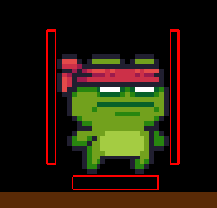
\includegraphics[width = 0.7\textwidth]{Imagenes/CollDetector.png}
	\caption{Representación de las cajas de detección de colisiones del jugador}
	\label{fig:Player_Coll_Detector}
\end{figure}
\subsubsection{PlayerBetterJumping}

Para que el salto se ajuste más al estándar de los juegos de plataformas 2D, este script mejora la sensación de salto para que el personaje caiga más rápido, evitando una sensación de flotación. Además, permite realizar saltos más pequeños si el jugador suelta el botón antes.\\
Para lograrlo, el script ajusta dos multiplicadores: uno que incrementa la gravedad cuando el jugador está cayendo y otro que reduce la altura del salto cuando este es interrumpido antes de tiempo.\\

\subsection{Life}

Se ha implementado una clase Life que gestiona los puntos de salud del objeto al que está adjunto y que se encarga de eliminar el objeto en el caso que su vida llegue a cero. El componente pedirá al usuario un valor inicial para los puntos de vida del objeto.\\
Este componente está estrechamente ligado al \textit{DamageSensor} el cual será mencionado más adelante y que detecta si ha habido una colisión con un objeto que aplique daño, esta relación es necesaria ya que para que se detecte el daño que decrementa la salud del objeto se necesita este sensor, por lo que al añadir un componente \textit{Life} se añadirá este sensor automáticamente.\\
\textit{Life} diferencia entre enemigos y el jugador, en caso de que el componente esté adjunto al jugador se deberá marcar en la opción \textit{EntityType} y el componente requerirá que se le de la referencia a un texto del \textit{Canvas} donde se escribirá la vida actual del jugador.\\

\subsection{PlayerDistanceAttack}

Componente encargado de representar un posible ataque a distancia del jugador. El ataque se activará con el clic izquierdo del ratón, lo que instanciará el prefab \textit{Bullet Prefab}, el cual implementa el comportamiento de una bala. La dirección que tomará la bala será aquella en la que se encuentre el cursor del ratón en el momento del clic.

Para evitar que el jugador pueda disparar sin restricción, se ha introducido un tiempo de espera entre disparos.\\

\section {FSM}

El comportamiento de la entidad estará encapsulado en una FSM, cuya única funcionalidad es la de gestionar el estado actual, comprobar que no ha habido ningún cambio de estado y, en caso de haberlo, manejar el cambio de estado.\\
Esta comprobación se hará al finalizar la actualización del estado actual (en el \textit{LateUpdate}) para así evitar problemas con cambiar de estado en medio de un bucle sin terminar.

\subsection{SensorStatePair}
Esta clase representa una transición de estado. Está compuesta por un sensor y un estado objetivo.\\
Si el sensor se activa, la entidad cambiará automáticamente al estado especificado.\\

\subsection{State}

La clase \textit{State} representa un estado de comportamiento de un enemigo. Para ello gestiona dos elementos fundamentales: \textit{Actuators} y \textit{Sensores}.\\

\begin{itemize}
	 \item Actuators: son actualizados en cada bucle y representan acciones.
	\item Sensors: pueden ser activados, lo que supone un cambio de estado al estado objetivo asociado en \textit{SensorStatePair}.
\end{itemize}
Cuando se produce un cambio de estado, todos los actuadores y sensores se detienen, y los sensores se desuscriben de todos los eventos a los que estuvieran vinculados.\\

\section{Actuators}

Como se ha mencionado anteriormente, un actuator es el script encargado de ejecutar una acción, por lo que para cada tipo de acción existirá un actuator que la represente.
La clase \textit{Actuator} representa la clase base de la que heredarán todos los tipos de actuadores.
Esta clase contiene métodos abstractos para iniciar, actualizar y destruir un actuador. Al ser abstractos cada clase que herede de \textit{Actuator} deberá implementar estos métodos.\\

\subsection{MovementActuators}
Movement contenido a ver si sale guay
\subsubsection{AAAA}
aaaaa
\subsection{Spawner}
Spawner
\section{Sensors and emitters}
Contenido
\subsection{Sensors}
mas contenido
\subsection{Emitters}
muchisimo mas
